\begin{figure*}[t]
\centering
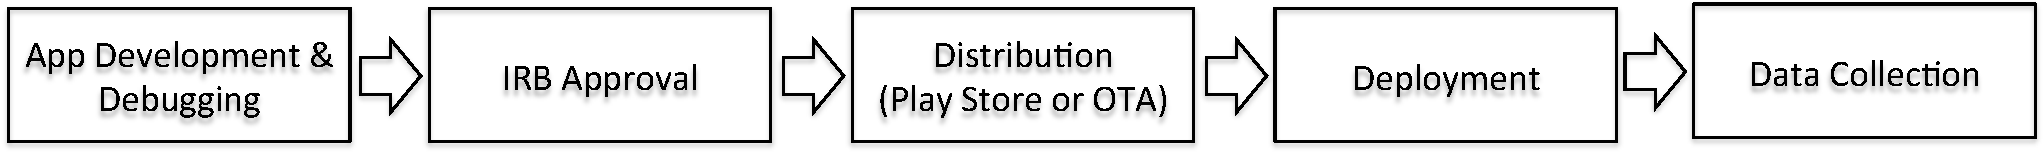
\includegraphics[width=0.9\textwidth]{experiment-life-cycle.pdf}
\caption{Expected Life Cycle of a \PhoneLab{} Experiment}
\label{fig:experiment-life-cycle}
\end{figure*}

\section{Experiment Case Study}
\label{sec-experiment}

We have conducted a measurement study to demonstrate the power of \PhoneLab{};
we have developed a logging tool, deployed it on 88 participant phones, and
collected data for 21 days. As mentioned in Section~\ref{sec:comparison}, the
reason why we decided to conduct a measurement study is because it requires a
combination of many features of \PhoneLab{}, e.g., scale, realism, timeliness,
and participant control. In a sense, a measurement study ``stress tests'' the
power of \PhoneLab{}.

We first give a look into how an experiment can be performed on \PhoneLab{} by
describing the expected life cycle of an experiment.
Figure~\ref{fig:experiment-life-cycle} overviews an expected life cycle of an
experiment. We then report how our own experiment proceeded for each step of the
life cycle.

\subsection{Experiment Life Cycle}

A typical \PhoneLab{} experiment will proceed in the following five steps.

{\bf App Development and Debugging:}
We expect that \PhoneLab{} users do a thorough job of local development and
debugging. \PhoneLab{} is not designed to be a debugging facility. Experimenters
should treat each app as a final product. Distribution via Play Store will help
in this regard because it imparts the sense that it is a product released to the
public. Not doing thorough debugging is not good for researchers either because
we cannot force our participants
to participate in any particular experiment if they are not comfortable 
participating, buggy or battery hungry software will annoy participants because
it disrupts the normal phone usage and will likely not participate.

{\bf IRB Approval:} Perhaps the biggest difference between \PhoneLab{} and other
existing testbeds is the requirement for IRB approval. Other testbeds only deal
with machines, no need for IRB. We deal with people, and protecting our
participants is one of our primary concerns. Because of this, we require each
experiment to go through the IRB approval process. This should be local for each
institution. SUNY Buffalo does not involve in this process. We will need to get
a copy of the approval or a letter describing the irrelevance of IRB approval.
We will only approve an experiment with this record.

{\bf Distribution:} App distribution is done via Play Store. Platform
distribution will be done via our infrastructure OTA. We initially explored the
option of using our infra to distribute apps, but realized that Play Store
provides all features we need for app distribution, e.g., automatic update. 

{\bf Deployment:} One the app is up on the Play Store, the experiment notifies
us and we notify our participants. Deployment is done by each participant by
installing the app from the Play Store. They will examine the permissions
requested and descriptions of the experiment. They might directly contact the
experimenters with questions.

{\bf Data Collection:} Data collection can happen in two ways, by using our data
collection with tags or by doing their own. Energy is a precious resource.

\subsection{Our Experiment}

{\bf App Development and Debugging:} Tool description. What we collect and where
we get it. Say that we're doing something similar to PowerTutor for battery
using Java reflection for fuelgauge. Comprehensive collection of information
(list them). 15 min interval to reduce power consumption. Power was the main
concern for our development.

{\bf IRB Approval and Distribution:} Started when and finished when. Delay is
mainly because of us. IRB side review itself took (how long). We uploaded our
first version on (date).

{\bf Deployment:} How long did it take to reach 88? Say that this in and of
itself is an experiment because we only sent out one mass email annoucing the
availability of the play store app.

{\bf Data Collection:} How much did we generate?
